%!TEX root = ../main.tex
%=========================================================

\section{Design}

\subsection{Topic Table}

\subsection{Tickets}
In order to place an ad on a registrar's topic table, the advertiser must present a valid 'ticket' to the registrar. Tickets are immutable objects issued by the registrars. An advertiser willing to register an ad at a registrar must first obtain a ticket from that registrar by sending a 'ticket request' (TICKETREQUEST) message to the registrar. In response to the ticket request, the registrar issues an initial ticket containing a 'waiting time' and sends the ticket to the advertiser in a 'ticket response' message. The advertiser can come back to the registrar (to register an ad) after the waiting time has elapsed and present the ticket in a 'topic registration request' (i.e., REGTOPIC) message.

Any REGTOPIC messages that are sent before the waiting time (indicated in the ticket) are ignored by the registrars. If the advertiser comes back to the registrar after the waiting time, the advertiser can either place the ad (and notify the advertiser of a successful registration) or issue another ticket with a new waiting time in another ticket response message. An advertiser may be given one or more tickets in a sequence before a successful registration, and this means that overall the advertiser waits for a 'cumulative waiting time' period that is the sum of multiple waiting times issued in each ticket in the sequence before finally registering an ad. Assignment of 'waiting times' is the only way the registrars can control the registrations in order to both:

\begin{itemize}
    \item Throttle ad placement rate to prevent overflowing of topic table: when the topic table is full, the advertisers must wait for already placed ads to expire first before they are allowed to register new ads.
    \item Prioritise registrations to achieve a diverse set of ads in the topic table. For example, registrations for less popular topics or registrations from advertisers that increase IP diversity (in the set of advertiser IP addresses that currently have an ad in the table) can be prioritised over others. This is useful to reduce the impact of Sybil attacks on the service discovery system.
\end{itemize}

Waiting times will be calculated according to a 'Waiting time function' (see below). Enforcing this time limit prevents misuse of the topic table because any topic must be important enough to outweigh the cost of waiting for ad placement. Imagine a group phone call: announcing the participants of the call using topic advertisement isn't a good use of the system because the topic exists only for a short time and will have very few participants. The waiting time prevents using the topic table for this purpose because the call might already be over before everyone could get registered. Also, it prevents attackers from overflowing topic table by regulating registrations in case of spamming attacks.

In addition to the waiting time, the sequence of tickets issued by a registrar for a specific advertiser also records the original issue-time of the first ticket which can be used to compute the cumulative waiting time so far; that is, the time elapsed since the advertiser requested its first ticket to place its ad. The inclusion of issue-time allows the registrars to prioritise advertisers that have been waiting the most as we explain later. Because the tickets are immutable (i.e., tampering with the ticket is detectable by the registrars that originally issued the ticket), when a registrar issues a new ticket (in case a registration is not immediately successful) to an advertiser, the registrar simply copies the issue-time from the last issued ticket and use that as the issue-time of the new ticket. This means that the registrars are not required to maintain any state for each on-going ticket request given that they can simply verify the authenticity of the ticket in the incoming registration requests. The registrars ensure the authenticity of the tickets they issue to the advertisers through symmetric encryption we explain below.

Tickets are immutable objects storing arbitrary information determined by the issuing registrar node. While details of encoding and ticket validation are up to the implementation, tickets must contain enough information to verify that:
\begin{itemize}
    \item The advertiser attempting to use the ticket is the one which originally requested it.
    \item A ticket is valid for a single topic only.
    \item A ticket can only be used within the 'registration window' (explained below).
    \item A ticket can't be used more than once.\michal{Can we enforce it? I can use the same ticket twice within the validity period, right?}
\end{itemize}

Tickets cannot be used beyond their lifetime. If an advertiser does not come back after the waiting time, all cumulative waiting time is lost and the advertiser must start over (\Cref{fig:ticket_validity}). When the ticket is issued, the node keeping it must wait until the registration window opens. The length of the registration window is implementation dependent, but by default 10 seconds is used. The ticket becomes invalid after the registration window has passed. This mechanism prevent from malicious advertisers who could get ticket, wait for a long time generating high cumulative waiting time and launching a coordinated attack to take over the topic table.
    
    
\begin{figure}
    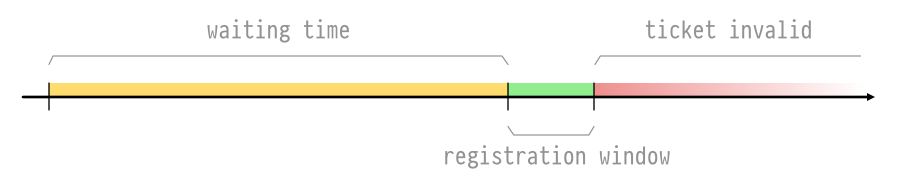
\includegraphics[width=0.5\textwidth]{img/ticket-validity}
    \caption{Ticket validity period.}
    \label{fig:ticket_validity}
\end{figure}

\subsection{Ticket Table}
The above description explains the storage and placement of ads on a single registrar, but the advertisers need to distribute ads redundantly on multiple nodes in order to speed up its discovery and to be discovered by more searchers at once. The main goal of distributing advertisements to be found within the network. An important issue is how advertisers distribute their ads among registrar nodes. Since every node may act as an advertisement medium for any topic, advertisers and searchers looking for ads must somehow meet at common registrars. Ideally, the topic search should be fast even when the number of advertisers for a topic is much smaller than the number of all live nodes. Given that in a decentralised setting, advertisers and registrars can not apriori agree on a subset of nodes to serve as the advertisement media for the topics, the main challenge for nodes is to find the "right" set of nodes to send advertisements and topic search queries so that they quickly meet at common nodes.



In order to execute the ad distribution process described below, each advertiser maintains a per-topic 'ticket table' for each topic it is advertising to keep track of the ongoing registration attempts with different registrars. This table is similar to the routing table used in Kademlia protocol, but instead of storing nodes based on distance for routing purposes, nodes are stored based on distance to topic ID to keep track of on-going registrations.

This table is made up of k-buckets of logarithmic distance to the topic hash (topic ID), i.e. the table stores k registrars for every distance step (bucket). It is sufficient to use a small value of k such as k=3. For this table no replacement list is used, different from the Kademlia routing table. Ticket table buckets are filled from the local routing table (Kademlia DHT Table) with the same distance to the topic hash.

Every node stored in the ticket table is a potential registrar. The advertiser attempts to place an ad on each registrar and keeps the latest ticket issued by that registrar. It also keeps references to all pending tickets in a priority queue keyed by the expiry time of the ticket so it can efficiently access the next ticket for which a placement attempt is due.

In our approach, advertisers start a limited number of parallel registrations in each ticket table bucket distance. More specifically, an advertiser follows the below steps to distribute its ads for a specific topic:
\begin{enumerate}
    \item The advertiser selects a set of K registrar nodes from each bucket distance of the ticket table structure, where the number of bucket distances (B) is a configurable parameter of the ticket table.
    \item A TICKETREQUEST message is initially sent to each of the selected registrar nodes in the previous step.
    \item Registrar node replies with a TICKETRESPONSE. This message includes the TICKET which contains a waiting time and a ticket issue time.
    \item The advertiser replies after the waiting time expires with a REGTOPIC request containing the previously received TICKET attached to it.
    \item A registration is successful when the waiting time calculated at the registrar is smaller than the cumulative waiting time, which means that the advertiser has waited long enough.The registrar sends a \item REGCONFIRMATION response to the advertiser. In general, the topic table occupancy is guaranteed to always remain below the topic table capacity by the waiting time calculated: the waiting time function returns increasingly large values as the topic table space runs out; the waiting time becomes infinite in case there is no space.
    \item The registrar replies with a REGRESPONSE message containing a new TICKET (containing a new waiting time) in case the registration is not succesful.
    \item A registrar gives up and stops the registration process with a registrar (say R) upon either T unsuccessful registration attempts (i.e., after being issued T tickets in REGRESPONSE messages from the registrar without a REGCONFIRMATION) or receipt of a ticket with a waiting time larger than LARGEWAIT. In that case, the advertiser selects a new node located in the same bucket as R, and initiates a TICKETREQUEST (step 2).
    \item Similarly, expiration of a previously placed ad (i.e., after the passage of ad-lifetime upon receiving a REGCONFIRMATION message) also triggers TICKETREQUEST to a new node that is in the same bucket as R.
\end{enumerate}

The objective of the ad placement process described above is to establish and maintain K active (i.e., unexpired) registrations in each bucket distance. This objective is achieved by the advertisers setting a timer with a duration of ad-lifetime immediately upon the receipt of a REGCONFIRMATION from a node in a bucket b, and once the timer expires (after ad-lifetime passes) the advertiser starts a fresh registration with a node that is also located in bucket b. The ticket table is used to store the tickets obtained for each on-going registrations and to keep track of the expiration times of active registrations.

\subsubsection{Bucket refresh}

The Ticket table needs to be initialised and refreshed to fill up all the per-distance k-buckets. Ideally, all k-buckets should be constantly full, meaning that the advertisers place registrations at registrars in all distances to the topic hash. An option to fill up all k-buckets would be to send periodic lookups for the specific distance to the topic hash, but since there are some distances that tend to be empty in the id space, sending periodic lookups for the topic hash may create an additional overhead that can be too expensive and create too much traffic in the network. To avoid that, initially, the 'ticket table' k-buckets are filled performing local DHT routing table lookups to all distances to the 'topic hash' of the advertised topic.

In addition to that, every time a node sends a ticket or registration request, the registrar replies with the closest nodes to 'the topic hash' that it knows. This helps filling up k-buckets without sending additional lookups. Also, when performing topic search (sending lookups for specific topics), closest known nodes to 'the topic hash' are attached by the registrar node in the response.

There is also a refresh bucket process, similar to the Kademlia DHT table, where periodically a random bucket is checked for empty buckets. The refresh time used is $refresh_time=10$ seconds. During the refresh process, the empty slots can be filled from the local DHT table list, and optionally a lookup (Kademlia FINDNODE) can be performed towards the topic hash. Also, all nodes in the bucket are periodically pinged to check they are still alive. In case they are not, tickets for those dead nodes are removed from the ticket table and registrations to new nodes are initiated.


\subsection{Waiting Time}
Waiting time function is used to calculate the waiting time reported to registering advertising nodes to regulate and control the ticket registration. The function directly shapes the structure of the topic table, determines its diversity and performs flow control. The function should also protect against all kinds of attacks, where a malicious actor tries to exhaust resources of the registrar. At the same time, no hard limits on the advertiser IPs/IDs/registered topic should be imposed, allowing the table to be used in various environments.

The waiting for a specific request follows the formula below (we assume that the ads contain advertiser IP, ID and topic):


\begin{equation}
    w=((\frac{1}{10^9}) + (\frac{d(IP)}{d})^{P_{IP}}+(\frac{d(ID)}{d})^{P_{ID}} (\frac{d(topic)}{d})^{P_{topic}}) \frac{ba}{(1-\frac{n}{d})^{P_{occupancy}}}
\end{equation}

All the modifiers from the first part of the equation increase with increasing number of the same items that are already in the table, i.e., reduction in diversity. Thus it's getting increasingly difficult to register ads for the same IP/ID/topic. For instance, ads for less popular topic will receive lower waiting times than popular ones. Note that the table does not prevent anyone from registering, but rather makes it slower for already popular items. Such a mechanism promotes diversity in the table and protects against Sybil attacks so that an attacker who is in control of a limited pool of IP addresses won't be able to dominate the table with many ads. The low exponent for the topics is motivated by the topics in the network that are likely to follow a skewed (e.g., a zipf-like) distribution. In contrast, honest nodes' IPs/IDs should follow a uniform distribution.

The latter part of the formula is determined based on a multiple of ad-lifetime and the current utilisation (i.e., occupancy divided by capacity) of the table. When the utilisation becomes closer to 1.0, the base time becomes very large due to a very small denominator. Before the waiting time becomes infinite (when utilisation becomes 1), the waiting time becomes extremely high, in which case the advertisers give up as explained in the ad distribution process.

\subsubsection{Lower Bound}

With the formula above, user are incentivized to keep checking the waiting time as frequently as possible hoping for a better one. An advertiser may get a better waiting time at t2 if an contribuing to the waiting time received at t1 (t1 < t2) expires before t2. One solution to this problem is to take into account all the expiration times when calculating the waiting time. However, such a solution is computationally expensive (O(n)) and unfeasible in practice.

We thus enforce a lower bound on the waiting time. I.e., we make sure that a searcher's waiting time received at t2 is not smaller than the waiting time at t1 by more than w(t1) - w(t2) < t2 - t1. To achieve that we split the above formula into topic/IP/ID distinctive parts:



The waiting time is equal to: 

For each of the components above IP, ID and topic present in the table, we keep a bound. When a specific IP enters the table for the first time, the bound(IP) is set to 0 and a timestamp timestamp(IP) is set to the current time. When a ticket request arrives from the same IP, we calculate the IP waiting time $w_{IP}$ and return the higher value among $w_{IP} = max(w_{IP}, bound(IP) - timestamp(IP))$. It makes sure that advertisers never receive a better time by frequently coming requesting new tickets. The bound and the bound are updated when a new ticket is issued and $w_{IP} > (bound(IP) - timestamp(IP))$. The same holds for IDs and topics.


\subsection{Topic Lookup}
The purpose of placing ads is to be discovered by searchers. Searchers maintain a separate table that they use to keep track of on-going searches called the 'search table'. Similar to the 'ticket table', the search table also stores k-buckets of advertisement media by distance to the topic hash, and a new 'search table' is created for each topic lookup. The k factor of the search table should be relatively large in order to make the search efficient. By default we use k=16 similarly to the Kademlia DHT. Tickets are not required for search and nodes can not be added multiple times in the same k-bucket.

To find ads, the searcher simply queries the nodes in the search table for ads. In order to find new results, bucket entries are replaced when the node fails to answer or when it answers with an empty list of ads. Bucket entries of the search table should also be replaced whenever the table is refreshed by a lookup.

\subsubsection{Search strategy}

For the lookup process, we perform ALPHA=3 parallel lookups to three different nodes. In case not enough LOOKUP\_LIMIT=50 results have been received for the first ALPHA lookups, additional ALPHA parallel lookups are performed until reaching LOOKUP\_LIMIT or MAX\_LOOKUP\_HOPS=50. We implemented and evaluated the following strategy in order to choose which nodes from which buckets ask first when performing a lookup. A random node is picked from a bucket following a round-robin approach. It starts picking a random node from the highest distance bucket and follows to the next distance in the bucket list.

\subsubsection{Bucket refresh}

Similarly to 'ticket table', 'search table' needs to be initialised and refreshed to fill up all the per-distance k-buckets. Ideally, all k-buckets should be constantly full, making it possible to query any distance to the topic hash. Since there are some distances that tend to be empty in the id space, sending periodic lookups for the topic hash my create and additional overhead that can create too much traffic in the network. To avoid that, initially, 'search table' k-buckets are filled performing local DHT routing table lookups to all distances to the 'topic hash'. In addition to that, every time an advertiser sends a ticket request and when performing topic search at a registrar, the registrar replies with the closest nodes to 'the topic hash' that it knows, helping to fill up the k-buckets of ticket tables without advertisers sending additional (Kademlia FINDNODE) lookups.

There is also a refresh process, similar to the Kademlia DHT table, where periodically a random bucket is checked for empty buckets. The refresh time used is refresh\_time=10 seconds. When empty slots during the refresh process, optionally, lookups are performed to the topic hash in case is empty. Also, the last node in the bucket is pinged to check it is still alive. In case it is not, it is removed from the table.